\documentclass[aspectratio=169,10pt]{beamer}

% ---------------------------------------------------------------- look
\usepackage[T1]{fontenc}
\usepackage[scaled=0.92]{helvet}
\renewcommand{\familydefault}{\sfdefault}
\usepackage{booktabs,tabularx,array,graphicx,xcolor,amsmath}
\usepackage{tikz,pgfplots}
\usetikzlibrary{positioning,arrows.meta,fit,calc}
\pgfplotsset{compat=1.17}
\graphicspath{{../results/figures/}{../results/figures/background_shift/}{../results/figures/birdshift_training/}{../results/figures/geography/}{img/}}

\definecolor{ink}{HTML}{111111}
\definecolor{muted}{HTML}{6B7280}
\definecolor{accent}{HTML}{C0392B}
\definecolor{good}{HTML}{15803D}
\definecolor{boxbg}{HTML}{F3F4F6}

\newcommand{\serif}{\fontfamily{ppl}\selectfont}
\setbeamertemplate{navigation symbols}{}
\setbeamercolor{normal text}{fg=ink,bg=white}
\setbeamercolor{frametitle}{fg=ink,bg=white}
\setbeamercolor{framesubtitle}{fg=ink}
\setbeamercolor{structure}{fg=ink}
\setbeamerfont{frametitle}{size=\fontsize{26}{28}\selectfont,family=\serif}
\setbeamerfont{framesubtitle}{size=\Large,family=\serif}
\makeatletter
\setbeamertemplate{frametitle}{%
  \vspace*{0.15cm}%
  {\usebeamerfont{frametitle}\usebeamercolor[fg]{frametitle}\insertframetitle}\par
  \ifx\insertframesubtitle\@empty\else
    \vspace{0.12cm}{\usebeamerfont{framesubtitle}\insertframesubtitle}\par
  \fi
  \vspace{0.05cm}}
\makeatother
\setbeamertemplate{footline}{%
  \hfill{\scriptsize\color{muted}\insertframenumber}\hspace*{0.45cm}\vspace*{0.3cm}}
\setbeamertemplate{itemize item}{\raisebox{0.15em}{\scalebox{0.7}{\textbullet}}}
\setbeamertemplate{itemize subitem}{\textendash}
\setbeamercolor{itemize item}{fg=muted}
\setbeamersize{text margin left=0.75cm,text margin right=0.75cm}
\setlength{\leftmargini}{1.1em}

\newcommand{\hl}[1]{\textcolor{accent}{#1}}
\newcommand{\up}[1]{\textcolor{good}{#1}}
\newcommand{\aside}[1]{{\footnotesize\color{muted}#1}}
\newcommand{\stat}[2]{%
  \begin{minipage}[t]{\linewidth}\centering
    {\serif\fontsize{26}{28}\selectfont #1}\\[0.15cm]
    {\footnotesize #2}
  \end{minipage}}

\tikzset{
  blk/.style={draw=ink,rounded corners=2pt,align=center,font=\scriptsize,
              minimum height=1.0cm,inner sep=4pt,fill=white},
  train/.style={blk,line width=1pt},
  fixd/.style={blk,dashed},
  shade/.style={blk,fill=boxbg},
  arr/.style={-{Stealth[length=5pt]},thick},
}

\begin{document}

% ================================================================ 1 title
{\setbeamertemplate{footline}{}
\begin{frame}
\begin{columns}[c]
\begin{column}{0.5\textwidth}
  {\serif\fontsize{44}{46}\selectfont BirdShift}\par\vspace{0.25cm}
  {\serif\Large\raggedright Context-Debiased Fine-Grained Bird Recognition under Geography,
  Background, and Long-Tail Shift\par}
  \vspace{0.35cm}
  {\small Progress report: experiments and results}\par\vspace{0.4cm}
  {\footnotesize DSE-312 Computer Vision\\ Instructor: Dr Samiran Das}\par\vspace{0.35cm}
  {\footnotesize Group members:}
  \begin{itemize}\footnotesize
    \item Shafwan Safi -- 24003
    \item Ankit Kumar -- 24045
    \item Agastya Bhanu -- 24025
  \end{itemize}
\end{column}
\begin{column}{0.46\textwidth}
  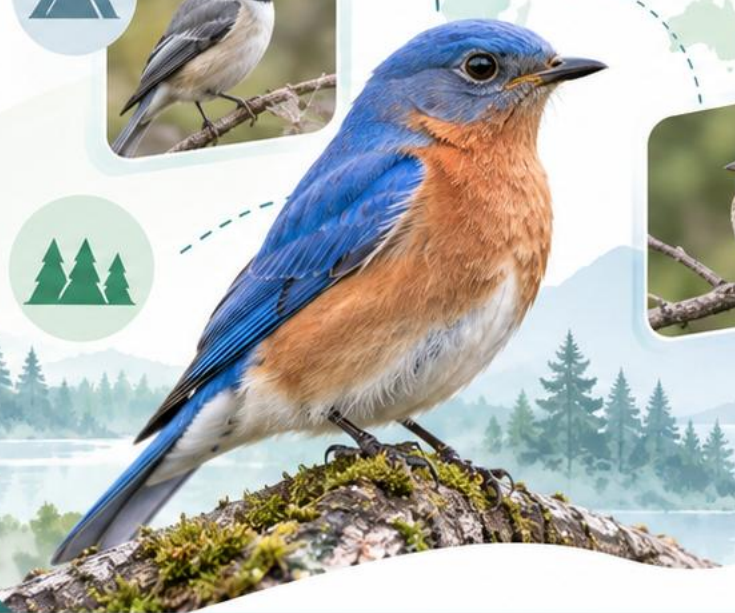
\includegraphics[width=\linewidth]{title-000.png}
\end{column}
\end{columns}
\end{frame}}

% ================================================================ 2 at a glance
\begin{frame}{At a glance}{What has been built and measured since the midterm}
\vspace{0.3cm}
\begin{columns}[t]
\begin{column}{0.24\textwidth}\stat{84.55\%}{CUB test top-1, ResNet-50 at 448\,px.\\Matches the published baseline (84.5\%)}\end{column}
\begin{column}{0.24\textwidth}\stat{$-$0.23\,pp}{BirdShift drop when the background is replaced\\(full image: $-$1.11\,pp)}\end{column}
\begin{column}{0.24\textwidth}\stat{23\,$\to$\,50\%}{Tail-class accuracy with logit-adjusted loss\\(+9.3\,pp overall)}\end{column}
\begin{column}{0.24\textwidth}\stat{56\,k}{iNaturalist images in a geography-held-out split, 154 species}\end{column}
\end{columns}
\vspace{0.7cm}
\begin{itemize}
  \item Three input variants trained and compared: \textbf{full image}, \textbf{bird crop}, \textbf{BirdShift} (background suppression during training).
  \item Controlled background-shift test set: original, blurred and replaced backgrounds on the same birds.
  \item Long-tailed CUB split (10:1) with four imbalance methods, reported by head / medium / tail.
  \item Training recipe fixed: torchvision weights + SGD + cosine LR gives \hl{+4.2\,pp} test over our first recipe.
\end{itemize}
\end{frame}

% ================================================================ 3 data
\begin{frame}{Data and splits}{One fixed protocol for every run}
\small
\begin{tabularx}{\linewidth}{@{}l >{\raggedright\arraybackslash}X r@{}}
\toprule
\textbf{Split} & \textbf{How it is built} & \textbf{Images}\\
\midrule
CUB train & 85\% of the official train split, stratified by species, seed 42 & 5,094\\
CUB val & remaining 15\%; used for all model selection & 900\\
CUB test & official test split, evaluated once after the recipe was frozen & 5,794\\
Long-tail train & exponential subsample of CUB train, 26 $\to$ 3 images per class & 2,039\\
iNat geo train / val & regions outside western North America; val = 15\% per species, whole outings & 31,161 / 5,510\\
iNat geo test & western North America, at least 100\,km from any training photo & 19,380\\
\bottomrule
\end{tabularx}

\vspace{0.3cm}
\begin{columns}[t]
\begin{column}{0.48\textwidth}
\textbf{Kept fixed}
\begin{itemize}\small
  \item ResNet-50 backbone (timm), 200-class head, seed 42
  \item Same val split for every run; checkpoint = best val accuracy
\end{itemize}
\end{column}
\begin{column}{0.48\textwidth}
\textbf{Metrics}
\begin{itemize}\small
  \item Top-1 and macro-F1
  \item Accuracy change under each shift; head / medium / tail accuracy
\end{itemize}
\end{column}
\end{columns}
\end{frame}

% ================================================================ 4 pipeline
\begin{frame}{Architecture and \hl{Pipeline}}
\centering
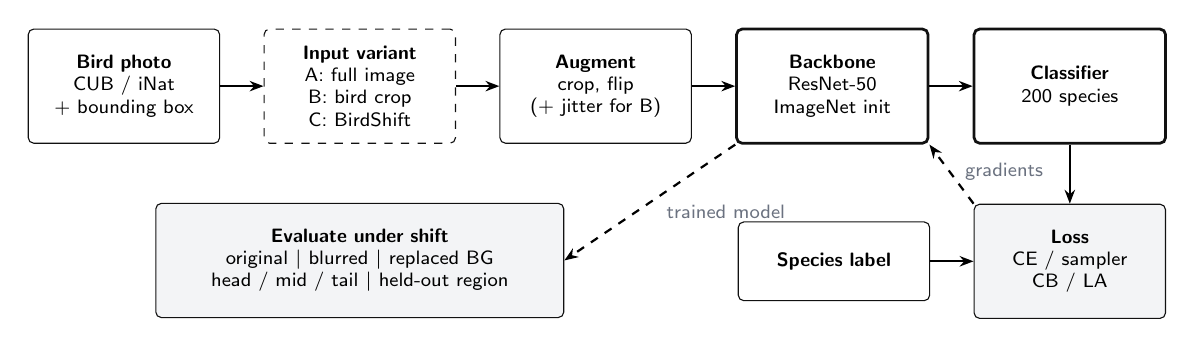
\begin{tikzpicture}[node distance=0.6cm and 0.55cm,
    every node/.append style={font=\small}, blk/.append style={minimum height=1.45cm, text width=2.15cm}]
  \node[blk] (img) {\textbf{Bird photo}\\CUB / iNat\\+ bounding box};
  \node[fixd, right=of img] (view) {\textbf{Input variant}\\A: full image\\B: bird crop\\C: BirdShift};
  \node[blk, right=of view] (aug) {\textbf{Augment}\\crop, flip\\(+ jitter for B)};
  \node[train, right=of aug] (bb) {\textbf{Backbone}\\ResNet-50\\ImageNet init};
  \node[train, right=of bb] (head) {\textbf{Classifier}\\200 species};
  \node[shade, below=0.75cm of head] (loss) {\textbf{Loss}\\CE / sampler\\CB / LA};
  \node[blk, left=of loss, minimum height=1.0cm] (lab) {\textbf{Species label}};
  \node[shade, below=0.75cm of view, text width=4.9cm] (eval) {\textbf{Evaluate under shift}\\original $|$ blurred $|$ replaced BG\\head / mid / tail $|$ held-out region};
  \draw[arr] (img) -- (view); \draw[arr] (view) -- (aug); \draw[arr] (aug) -- (bb);
  \draw[arr] (bb) -- (head); \draw[arr] (head) -- (loss); \draw[arr] (lab) -- (loss);
  \draw[arr,dashed] (loss.north west) -- node[pos=0.55,right=2pt,font=\scriptsize\color{muted}]{gradients} (bb.south east);
  \draw[arr,dashed] (bb.south west) -- node[pos=0.45,below right=-1pt,font=\scriptsize\color{muted}]{trained model} (eval.east);
\end{tikzpicture}

\vspace{0.25cm}
\begin{tabularx}{\linewidth}{@{}>{\raggedright\arraybackslash}X>{\raggedright\arraybackslash}X>{\raggedright\arraybackslash}X@{}}
\toprule
\textbf{BirdShift (variant C)} & \textbf{Imbalance methods} & \textbf{Speed-ups}\\
\midrule
\footnotesize Outside the box is blurred (radius 22) with $p=0.5$ per training image. No box is needed at test time.
& \footnotesize Weighted sampler, class-balanced CE ($\beta{=}0.999$), logit-adjusted CE ($\tau{=}1$), post-hoc LA.
& \footnotesize float16 mixed precision + \texttt{channels\_last}: 448\,px run in about 12 min on one RTX 3090.\\
\bottomrule
\end{tabularx}
\end{frame}

% ================================================================ 5 shift construction
\begin{frame}{Background shift}{Experiment 1: same bird, only the context changes}
\centering
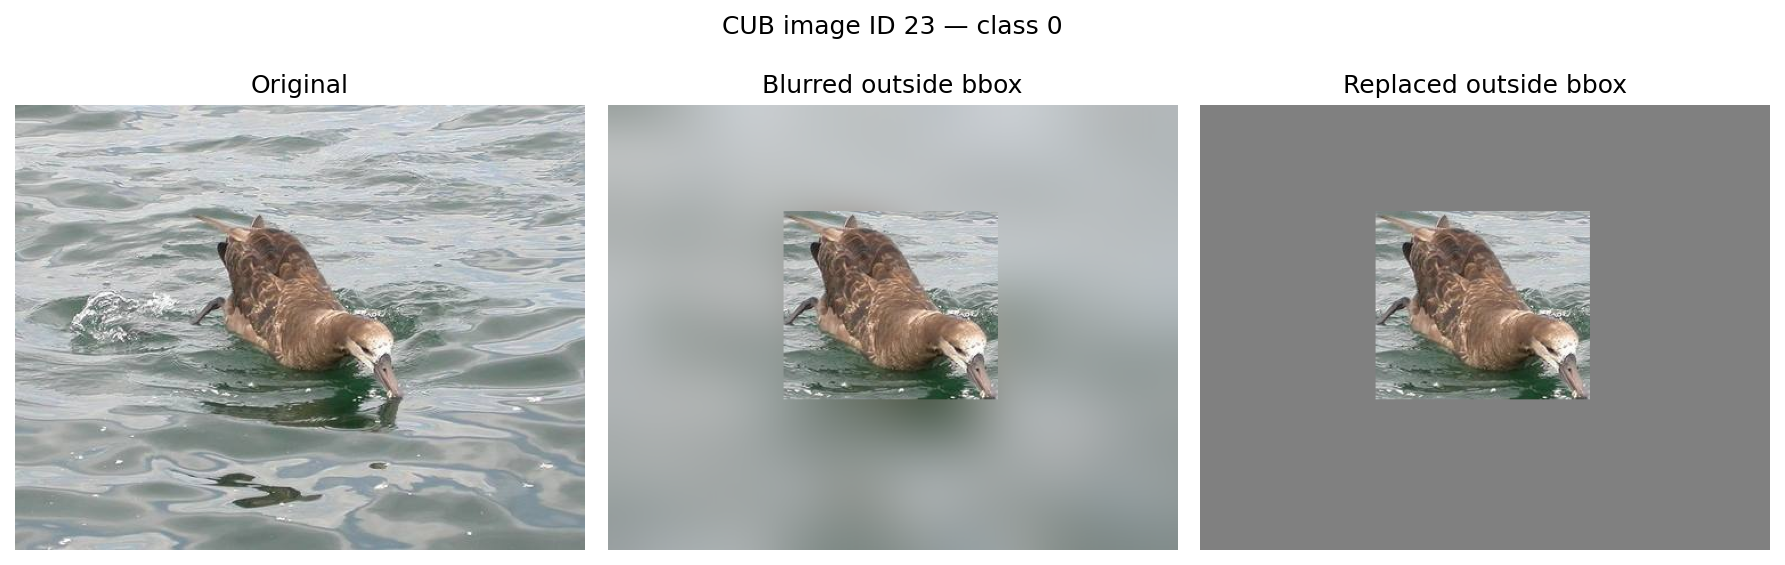
\includegraphics[width=0.92\linewidth,trim=0 0 0 75,clip]{image_23.png}

\vspace{0.3cm}
\begin{columns}[t]
\begin{column}{0.3\textwidth}\small\textbf{Original}\\ Normal evaluation. Reference accuracy.\end{column}
\begin{column}{0.3\textwidth}\small\textbf{Blurred background}\\ Gaussian blur (radius 22) outside the box. Colours stay, texture goes.\end{column}
\begin{column}{0.3\textwidth}\small\textbf{Replaced background}\\ Flat neutral gray. No donor photo, so no second bird or habitat can leak in.\end{column}
\end{columns}
\vspace{0.2cm}
\aside{If accuracy drops when only the background changes, the model was partly using the scene.}
\end{frame}

% ================================================================ 6 birdshift training
\begin{frame}{BirdShift training}{Break the link between background and label}
\centering
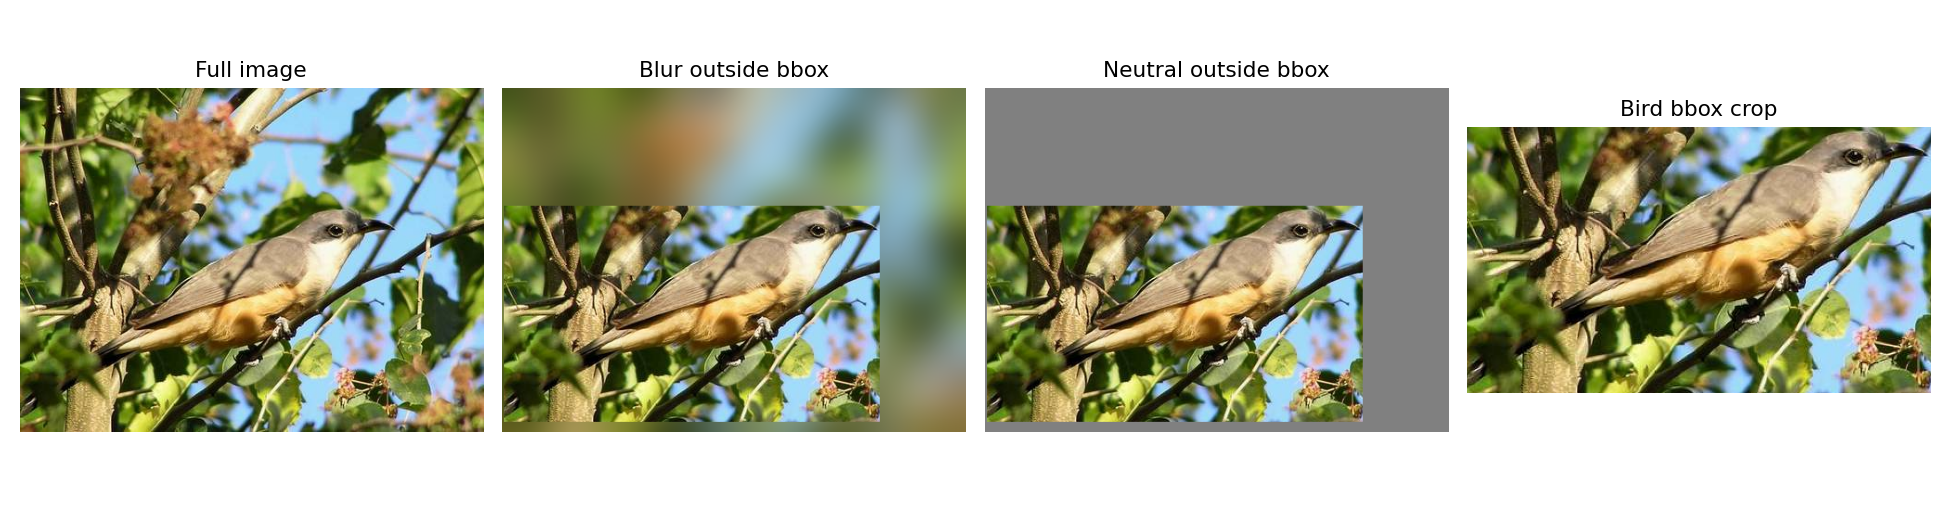
\includegraphics[width=0.95\linewidth,trim=0 40 0 40,clip]{image_1803.png}

\vspace{0.3cm}
\begin{columns}[t]
\begin{column}{0.47\textwidth}
\begin{itemize}\small
  \item Each training image: with probability 0.5 the area outside the bounding box is blurred.
  \item The model sees the same bird with and without its habitat, so the habitat stops being a reliable cue.
\end{itemize}
\end{column}
\begin{column}{0.47\textwidth}
\begin{itemize}\small
  \item At test time the input is the plain full image, like variant A.
  \item Bird crop (variant B) needs a box for every test image; BirdShift does not.
\end{itemize}
\end{column}
\end{columns}
\end{frame}

% ================================================================ 7 results 224
\begin{frame}{Results at 224\,px}{Experiment 1: top-1 on the 900 validation images}
\begin{columns}[c]
\begin{column}{0.5\textwidth}
\small
\begin{tabular}{@{}lccc@{}}
\toprule
\textbf{Model} & \textbf{Original} & \textbf{Blurred} & \textbf{Replaced}\\
\midrule
Full image & \textbf{78.33} & 77.33 & 76.67\\
Bird crop & 77.89 & 77.89 & 77.89\\
\textbf{BirdShift} & 78.22 & \textbf{78.78} & \textbf{77.78}\\
\midrule
\multicolumn{4}{@{}l}{\footnotesize\textit{Change from original (pp)}}\\
Full image & & \hl{$-$1.00} & \hl{$-$1.67}\\
Bird crop & & 0.00 & 0.00\\
BirdShift & & \up{+0.56} & $-$0.44\\
\bottomrule
\end{tabular}

\vspace{0.4cm}
\begin{itemize}
  \item Full image loses accuracy whenever the background changes.
  \item BirdShift matches it on normal photos ($-$0.11\,pp) and holds up under both shifts.
\end{itemize}
\end{column}
\begin{column}{0.48\textwidth}
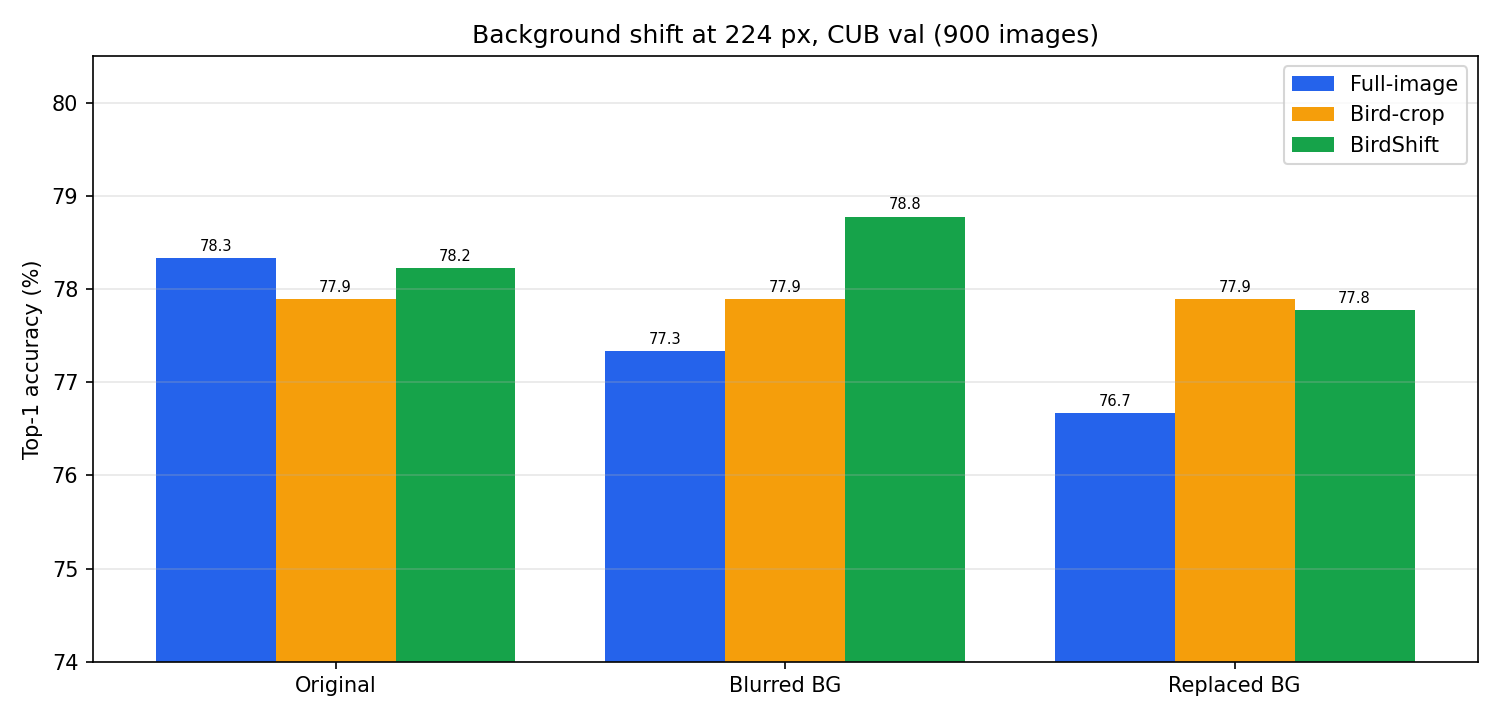
\includegraphics[width=\linewidth]{results_background.png}
\end{column}
\end{columns}
\end{frame}

% ================================================================ 8 results 448
\begin{frame}{Results at 448\,px}{Experiment 1: higher resolution, same conclusion}
\begin{columns}[c]
\begin{column}{0.5\textwidth}
\small
\begin{tabular}{@{}lcccc@{}}
\toprule
\textbf{Model} & \textbf{Orig.} & \textbf{Blur} & \textbf{Repl.} & \textbf{vs 224}\\
\midrule
Full image & 79.44 & 79.22 & 78.33 & +1.11\\
Bird crop & \textbf{81.33} & \textbf{81.33} & \textbf{81.33} & +3.44\\
\textbf{BirdShift} & 79.67 & 79.56 & 79.44 & +1.45\\
\midrule
\multicolumn{5}{@{}l}{\footnotesize\textit{Change from original (pp)}}\\
Full image & & $-$0.22 & \hl{$-$1.11} & \\
BirdShift & & \up{$-$0.11} & \up{$-$0.23} & \\
\bottomrule
\end{tabular}

\vspace{0.2cm}
\begin{itemize}
  \item Every model gains from 448\,px; the crop model gains most.
  \item Full image still drops most under replacement (10 images); BirdShift moves by 2.
  \item BirdShift beats full image in all three conditions.
\end{itemize}
\end{column}
\begin{column}{0.48\textwidth}
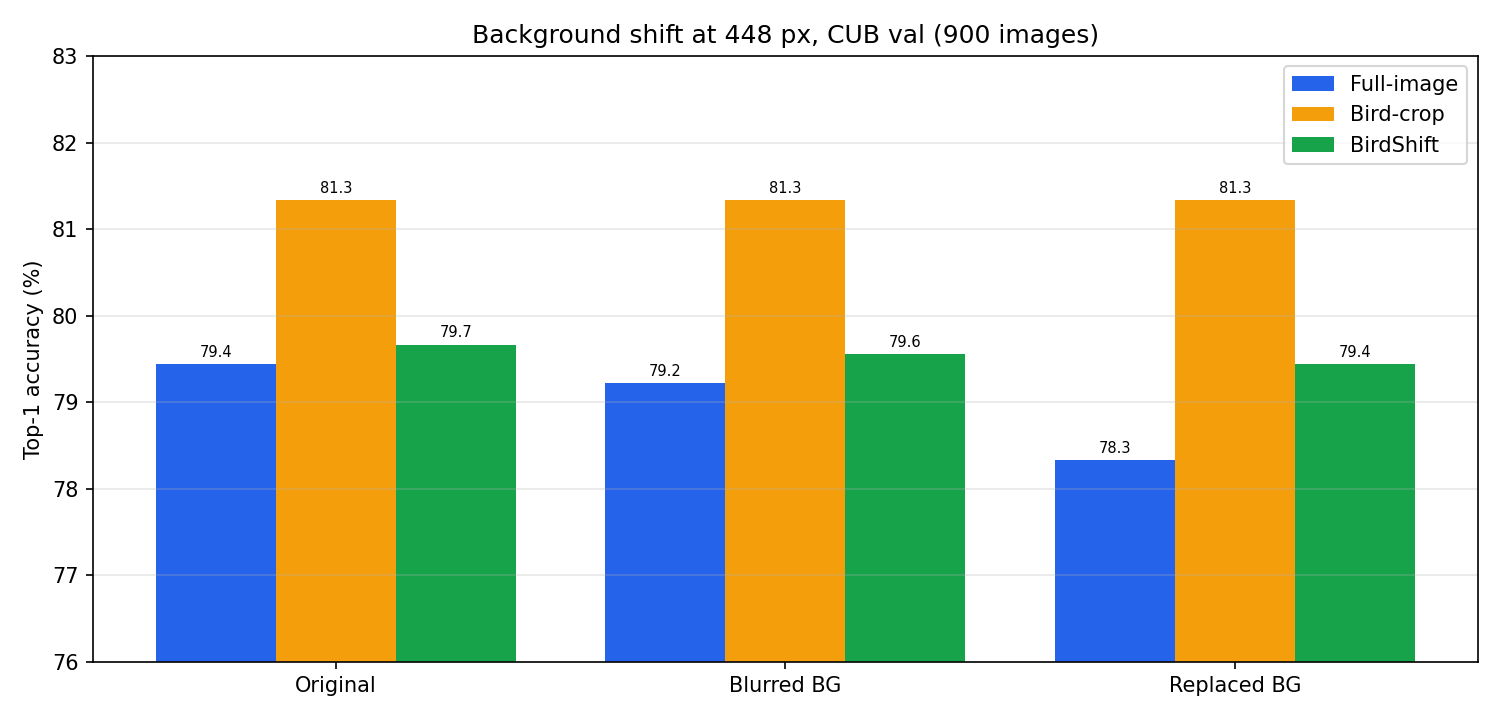
\includegraphics[width=\linewidth]{results_background_448.png}
\end{column}
\end{columns}
\end{frame}

% ================================================================ 9 recipe
\begin{frame}{Reaching the published baseline}{ResNet-50 at 448\,px, one change at a time}
\footnotesize
\begin{tabularx}{\linewidth}{@{}l l l l X r r@{}}
\toprule
\textbf{Run} & \textbf{Optimizer} & \textbf{Weights} & \textbf{Crop} & \textbf{Schedule} & \textbf{Val} & \textbf{Test}\\
\midrule
First recipe & AdamW $10^{-4}$ & timm a1 & RandomResizedCrop & constant, 30 ep & 79.33 & 80.38\\
+ crop, cosine & AdamW $10^{-4}$ & timm a1 & Resize 512 + crop 448 & cosine, 50 ep & 79.44 & 80.74\\
+ SGD & SGD 0.01, head $\times$10 & timm a1 & Resize 512 + crop 448 & cosine, 50 ep & 75.00 & 76.08\\
+ torchvision weights & SGD 0.01, head $\times$10 & torchvision & Resize 512 + crop 448 & cosine, 50 ep & \textbf{84.00} & \textbf{83.88}\\
\midrule
\textbf{Final: train + val} & \multicolumn{4}{l}{same recipe, all 5,994 training images, last epoch} & n/a & \hl{\textbf{84.55}}\\
\bottomrule
\end{tabularx}

\vspace{0.3cm}
\begin{columns}[t]
\begin{column}{0.48\textwidth}
\begin{itemize}
  \item \textbf{Pretrained weights were the main factor} (+7.8\,pp). timm's default weights come from a heavy-augmentation, BCE-loss recipe and transfer worse to birds [5, 6].
  \item SGD only helps together with the torchvision weights.
\end{itemize}
\end{column}
\begin{column}{0.48\textwidth}
\begin{itemize}
  \item Recipe chosen on val; test evaluated once at the end.
  \item Published reference: 84.5\% [3]. Model released as \texttt{v1.0} on GitHub.
\end{itemize}
\end{column}
\end{columns}
\end{frame}

% ================================================================ 10 recipe curves
\begin{frame}{Recipe search: training curves}
\centering
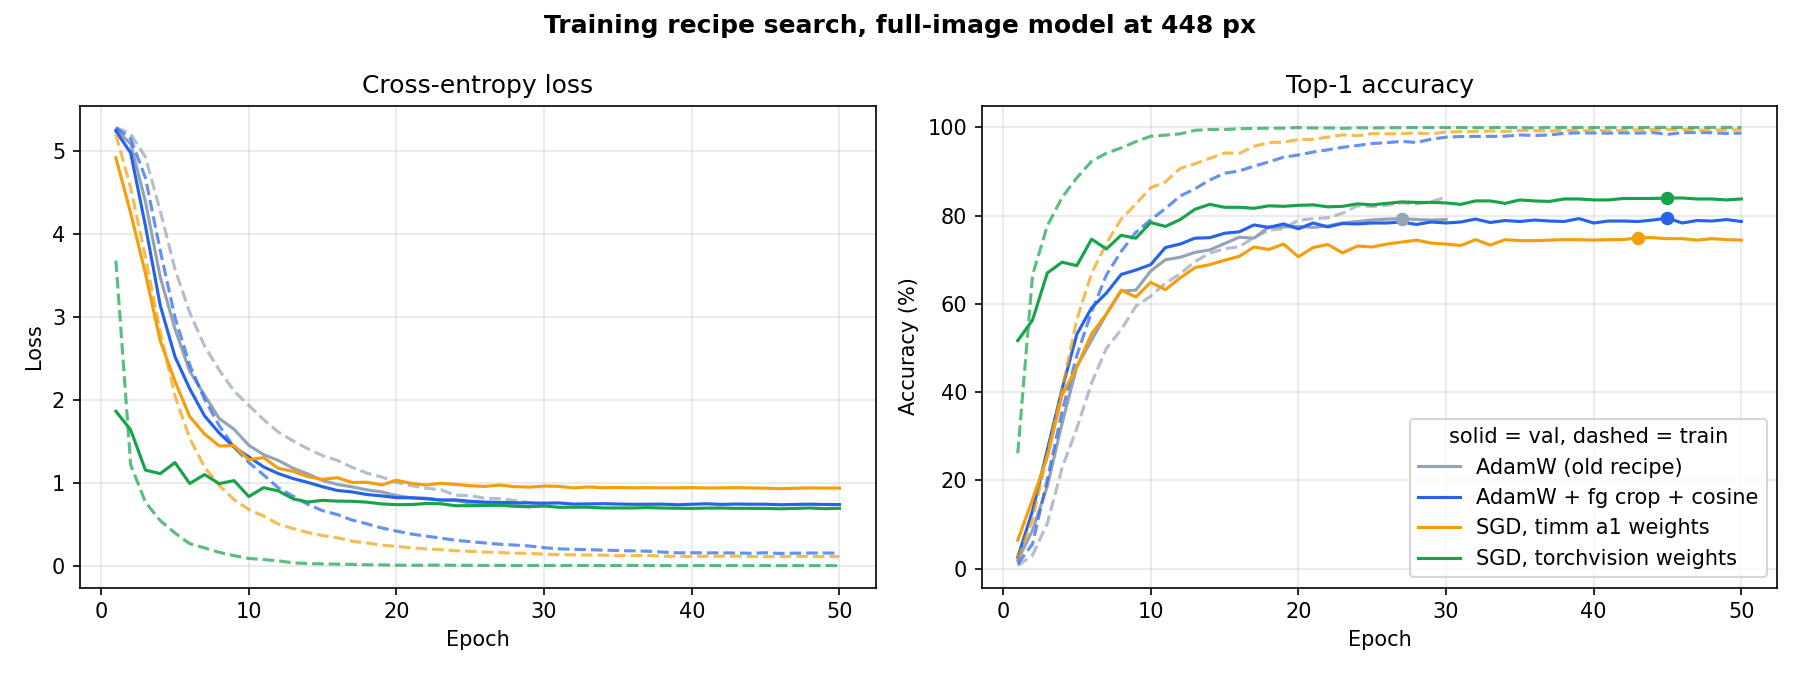
\includegraphics[width=0.97\linewidth]{curves_recipe.png}

\vspace{0.2cm}
\aside{Solid = validation, dashed = train, dot = best epoch. The torchvision-initialised run starts at 52\% val after one epoch and stays about 5\,pp above the others throughout.}
\end{frame}

% ================================================================ 11 long-tail setup
\begin{frame}{Class imbalance}{Experiment 2: CUB is balanced, so we make it long-tailed}
\begin{columns}[c]
\begin{column}{0.47\textwidth}
\centering
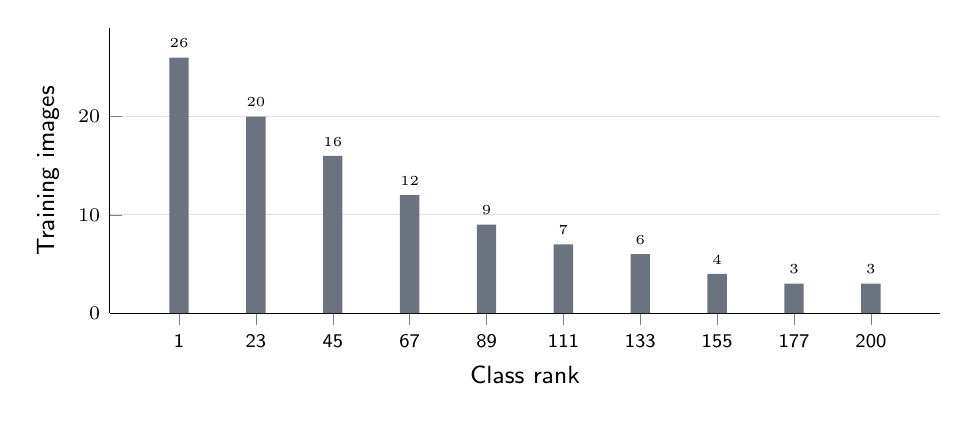
\begin{tikzpicture}
\begin{axis}[width=\linewidth,height=5.2cm,ybar,bar width=7pt,
  xlabel={Class rank},ylabel={Training images},ymin=0,ymax=29,
  symbolic x coords={1,23,45,67,89,111,133,155,177,200},xtick=data,
  tick label style={font=\scriptsize},label style={font=\small},
  axis lines*=left,ymajorgrids,grid style={gray!25},
  nodes near coords,every node near coord/.append style={font=\tiny}]
\addplot[fill=muted,draw=none] coordinates {(1,26) (23,20) (45,16) (67,12) (89,9) (111,7) (133,6) (155,4) (177,3) (200,3)};
\end{axis}
\end{tikzpicture}

\aside{$n_r = n_{\max}\cdot 10^{-r/199}$: 5,094 $\to$ 2,039 images. Classes shuffled first, so the tail is not one bird family. Val stays balanced.}
\end{column}
\begin{column}{0.5\textwidth}
\small
\begin{tabularx}{\linewidth}{@{}l X@{}}
\toprule
\textbf{Method} & \textbf{Idea}\\
\midrule
Standard CE & plain cross-entropy\\
Weighted sampler & sample image $i$ $\propto 1/n_{c(i)}$\\
Class-balanced CE & $w_c = \frac{1-\beta}{1-\beta^{n_c}}$, $\beta=0.999$ [2]\\
Logit-adjusted CE & train on $z + \tau\log\pi$, predict with $z$ [4]\\
Post-hoc LA & CE model, predict with $z - \tau\log\pi$\\
\bottomrule
\end{tabularx}

\vspace{0.3cm}
\aside{$\pi_c$ = share of training images in class $c$; $\tau=1$ as in the paper, not tuned. Head / medium / tail = thirds of classes by training count.}
\end{column}
\end{columns}
\end{frame}

% ================================================================ 12 long-tail results
\begin{frame}{Long-tail results}{Experiment 2: top-1 on the balanced validation set}
\begin{columns}[c]
\begin{column}{0.53\textwidth}
\footnotesize
\setlength{\tabcolsep}{4pt}\begin{tabular}{@{}lccccc@{}}
\toprule
\textbf{Method} & \textbf{Top-1} & \textbf{F1} & \textbf{Head} & \textbf{Mid} & \textbf{Tail}\\
\midrule
Standard CE & 53.00 & .477 & \textbf{80.20} & 56.39 & \hl{23.18}\\
Weighted sampler & 59.78 & .571 & 70.31 & \textbf{66.56} & 42.72\\
Class-bal.\ CE & 59.33 & .563 & 72.35 & 63.28 & 42.72\\
\textbf{Logit-adj.\ CE} & \textbf{62.33} & \textbf{.597} & 73.38 & 64.26 & \up{\textbf{49.67}}\\
Post-hoc LA & 59.67 & .567 & 74.74 & 63.61 & 41.06\\
\bottomrule
\end{tabular}

\vspace{0.4cm}
\begin{itemize}
  \item Plain CE: 80\% on common classes, 23\% on rare ones.
  \item \textbf{Logit-adjusted CE is best}: +9.3\,pp overall, tail accuracy more than doubled.
  \item Post-hoc LA needs no retraining and still gives +6.7\,pp.
\end{itemize}
\end{column}
\begin{column}{0.44\textwidth}
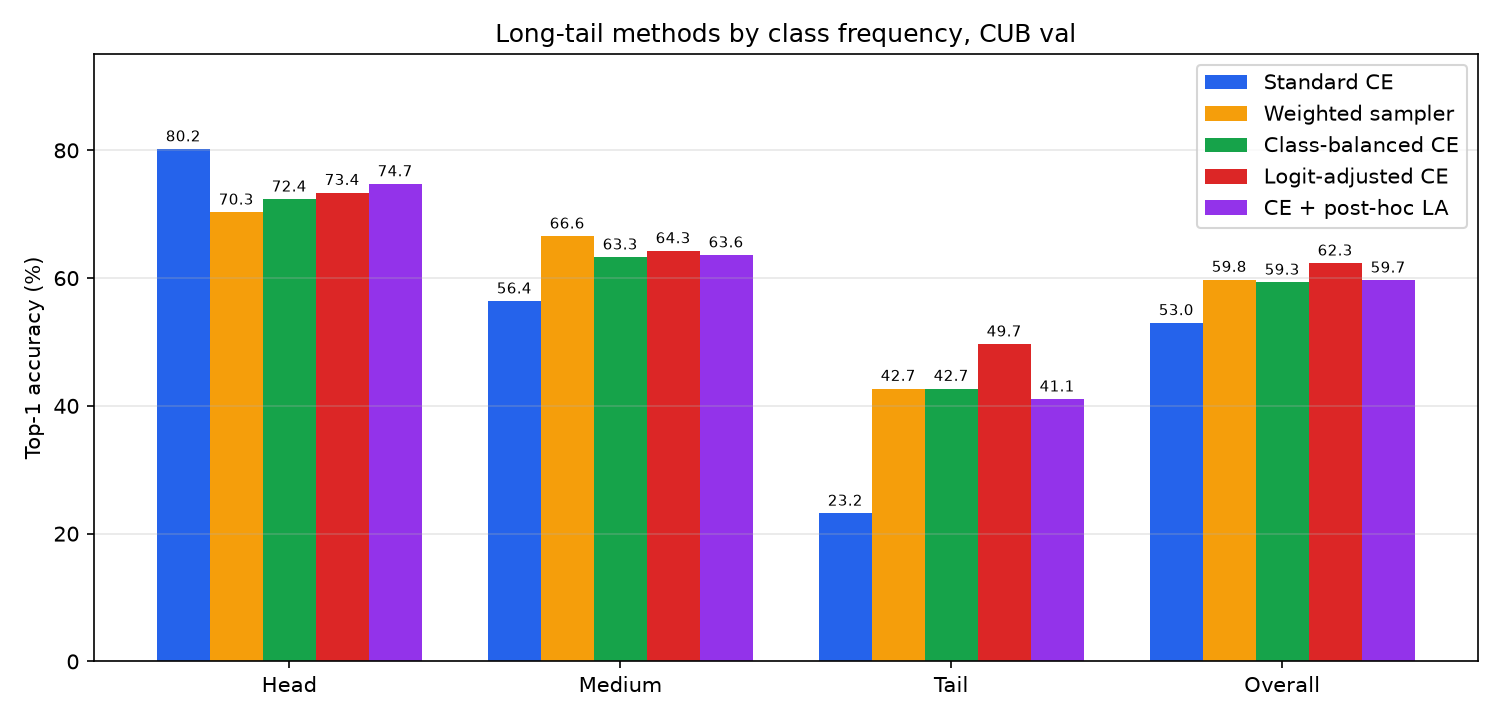
\includegraphics[width=\linewidth]{results_longtail.png}
\end{column}
\end{columns}
\end{frame}

% ================================================================ 13 geography
\begin{frame}{Geography split}{iNaturalist photos of CUB species (Ankit)}
\begin{columns}[c]
\begin{column}{0.55\textwidth}
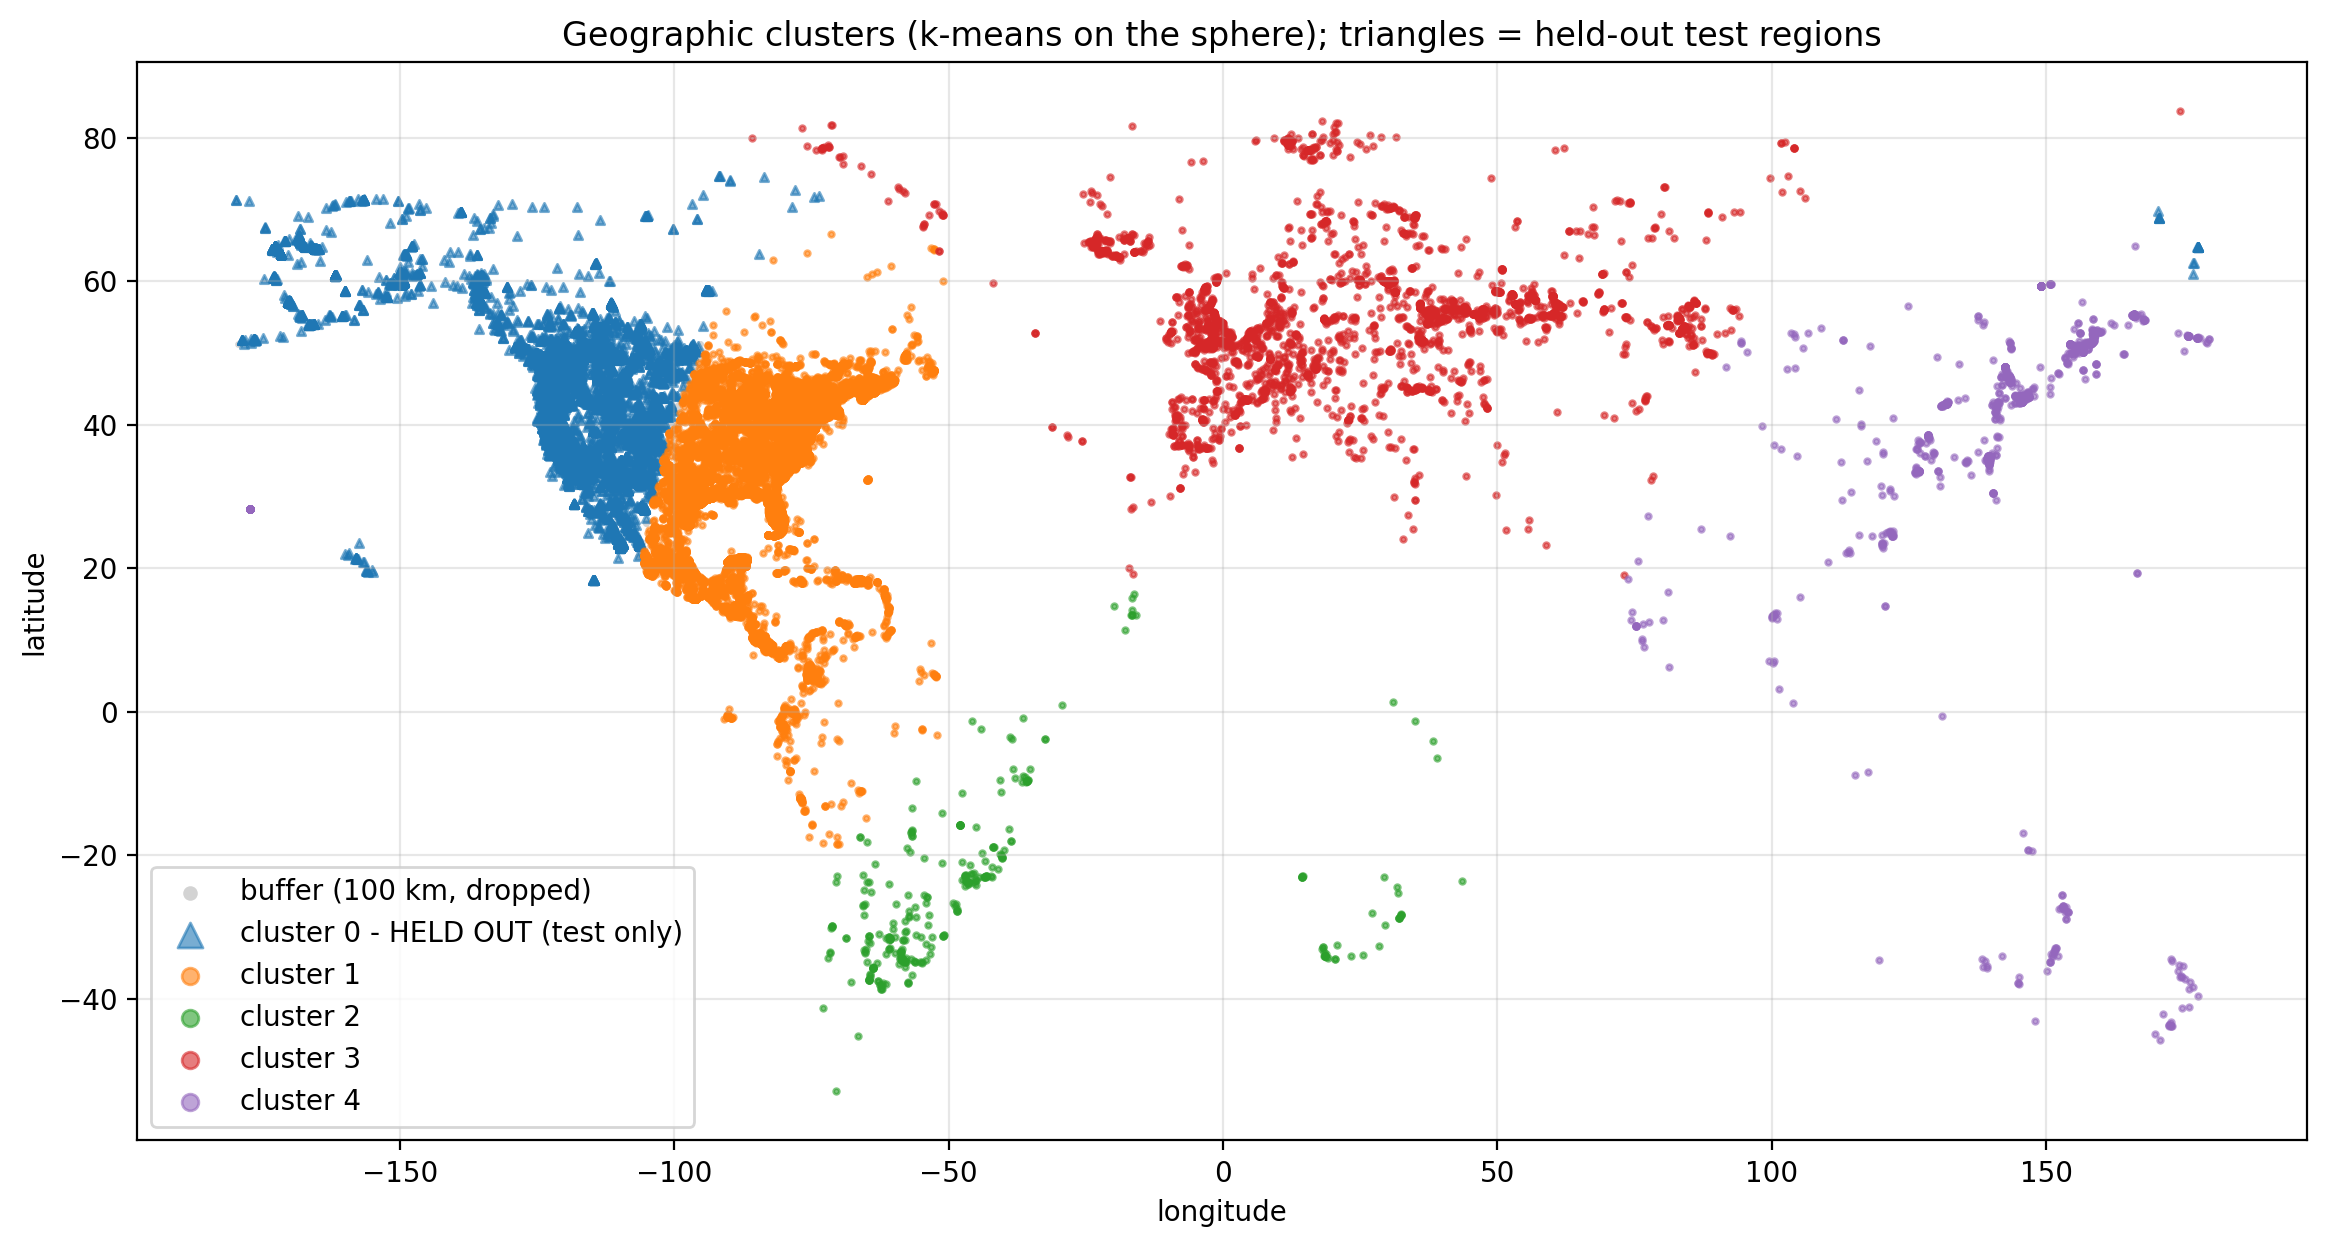
\includegraphics[width=\linewidth]{clusters_map.png}
\end{column}
\begin{column}{0.42\textwidth}
\small
\begin{itemize}
  \item Research-grade, CC-licensed, location within 10\,km.
  \item k-means ($k{=}5$) on lat/lon unit vectors.
  \item Test = western North America; 100\,km buffer removed from train/val.
  \item 154 of 200 species have $\geq$10 train and $\geq$5 test images.
\end{itemize}
\vspace{0.15cm}
\textbf{From the review}
\begin{itemize}
  \item 7 flock photos had 2--3 species labels: dropped.
  \item Myrtle Warbler mapping pulls in Audubon's Warbler: remap pending.
\end{itemize}
\end{column}
\end{columns}
\end{frame}

% ================================================================ 14 problems
\begin{frame}{Problems and fixes}
\footnotesize\renewcommand{\arraystretch}{1.45}
\begin{tabularx}{\linewidth}{@{}>{\raggedright\arraybackslash}p{4.1cm} >{\raggedright\arraybackslash}X >{\raggedright\arraybackslash}p{4.6cm}@{}}
\toprule
\textbf{Problem} & \textbf{How we noticed} & \textbf{Fix}\\
\midrule
Bird-crop model stuck at 40\% & Far below full image (78\%) & Pad crops to square before resizing, add augmentation: 40.3 $\to$ \textbf{77.9\%}\\
Two evaluators could disagree & Shift test must equal normal eval & Image-by-image audit: 0 mismatches\\
Replaced background could leak & Donor photos bring habitat or birds & Use flat neutral gray instead\\
BirdShift overwrote crop checkpoints & Wrong mode stored in a checkpoint & Removed override, one folder per run\\
CUB too balanced for imbalance study & 25--30 images per class & Seeded 10:1 long-tail subsample\\
4 pp below published ResNet-50 & 80.4\% vs 84.5\% on test & Ablation: torchvision weights + SGD $\to$ \textbf{84.55\%}\\
Same photo, several species (iNat) & Duplicate \texttt{photo\_id}s in review & Drop multi-label photos, assert uniqueness\\
\bottomrule
\end{tabularx}
\end{frame}

% ================================================================ 15 status
\begin{frame}{Current progress}
\begin{columns}[t]
\begin{column}{0.32\textwidth}
{\serif\Large Done}\par\vspace{0.15cm}
\begin{itemize}\small
  \item Full image, bird crop, BirdShift at 224 and 448\,px
  \item Background-shift test set and evaluation
  \item Long-tail split, 5 imbalance methods
  \item Recipe matching 84.5\% on CUB test
  \item Geography split (154 species, 56\,k images)
  \item Code, results and model on GitHub
\end{itemize}
\end{column}
\begin{column}{0.32\textwidth}
{\serif\Large In progress}\par\vspace{0.15cm}
\begin{itemize}\small
  \item Species-map corrections for the geography split (Ankit)
  \item Background clusters from real scenes (Agastya)
  \item Dataset loader for the iNaturalist manifest
\end{itemize}
\end{column}
\begin{column}{0.32\textwidth}
{\serif\Large Next}\par\vspace{0.15cm}
\begin{itemize}\small
  \item Rerun Experiments 1 and 2 with the SGD recipe
  \item Train full vs BirdShift on the geography split
  \item Logit adjustment + BirdShift together
  \item Test-split numbers, 3 seeds, paired significance tests
\end{itemize}
\end{column}
\end{columns}
\vspace{0.5cm}
\aside{All numbers so far: one seed (42); Experiments 1 and 2 on the 900-image val split, so 1\,pp = 9 images.}
\end{frame}

% ================================================================ 16 references
\begin{frame}{References}
\scriptsize
\begin{enumerate}\setlength{\itemsep}{2pt}
  \item[{[1]}] C. Wah et al. \textit{The Caltech-UCSD Birds-200-2011 Dataset.} Caltech, 2011.
  \item[{[2]}] Y. Cui, M. Jia, T.-Y. Lin, Y. Song, S. Belongie. \textit{Class-Balanced Loss Based on Effective Number of Samples.} CVPR 2019.
  \item[{[3]}] Z. Yang et al. \textit{Learning to Navigate for Fine-grained Classification.} ECCV 2018.
  \item[{[4]}] A. K. Menon et al. \textit{Long-Tail Learning via Logit Adjustment.} ICLR 2021.
  \item[{[5]}] R. Wightman, H. Touvron, H. J\'egou. \textit{ResNet Strikes Back: An Improved Training Procedure in timm.} NeurIPS 2021 Workshop.
  \item[{[6]}] S. Kornblith, J. Shlens, Q. V. Le. \textit{Do Better ImageNet Models Transfer Better?} CVPR 2019.
  \item[{[7]}] K. Xiao, L. Engstrom, A. Ilyas, A. Madry. \textit{Noise or Signal: The Role of Image Backgrounds in Object Recognition.} ICLR 2021.
  \item[{[8]}] K. He, X. Zhang, S. Ren, J. Sun. \textit{Deep Residual Learning for Image Recognition.} CVPR 2016.
  \item[{[9]}] P. Micikevicius et al. \textit{Mixed Precision Training.} ICLR 2018.
  \item[{[10]}] I. Loshchilov, F. Hutter. \textit{SGDR: Stochastic Gradient Descent with Warm Restarts.} ICLR 2017.
  \item[{[11]}] G. Van Horn et al. \textit{The iNaturalist Species Classification and Detection Dataset.} CVPR 2018.
\end{enumerate}
\vspace{0.3cm}
\aside{Code, results and the trained model: \texttt{github.com/Shafwansafi06/BirdShift}}
\end{frame}

\end{document}
